% ============================================================================
% Droites paralleles : (IJ) // (BC)
% Extrait de la fiche : Barycentres et lignes de niveau (classe de 1ere D)
% Necessite \usepackage{tikz} et \usetikzlibrary{calc} (charges par le fichier principal)
% ============================================================================
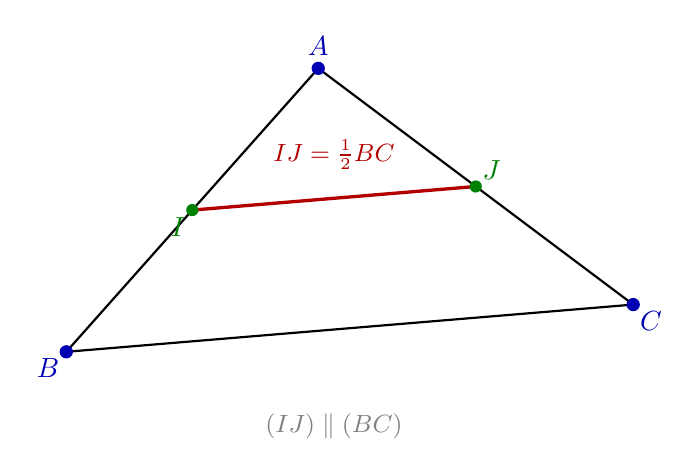
\begin{tikzpicture}[scale=1.0,>=latex]
  \coordinate (A) at (0.8,3.6); \coordinate (B) at (-2.4,0); \coordinate (C) at (4.8,0.6);
  \coordinate (I) at (-0.8,1.8); \coordinate (J) at (2.8,2.1);
  \draw[thick] (A) -- (B) -- (C) -- cycle;
  \draw[very thick,red!70!black] (I) -- (J);
  \fill[blue!70!black] (A) circle (2.4pt) node[above=1pt] {$A$};
  \fill[blue!70!black] (B) circle (2.4pt) node[below left=-1pt] {$B$};
  \fill[blue!70!black] (C) circle (2.4pt) node[below right=-1pt] {$C$};
  \fill[green!50!black] (I) circle (2.2pt) node[below left=-1pt] {$I$};
  \fill[green!50!black] (J) circle (2.2pt) node[above right=-1pt] {$J$};
  \node[red!70!black,font=\small] at (1.0,2.5) {$IJ=\frac{1}{2}BC$};
  \node[font=\small,gray] at (1.0,-0.95) {$(IJ)\parallel(BC)$};
\end{tikzpicture}
